\section{Lecture 3}
\begin{itemize}
    \item The absolute value is defined as
    \begin{equation}
        |a|=\begin{cases}
            +a \,& a \ge 0 \\ 
            -a, & a < 0
        \end{cases}
        \label{eq:}
    \end{equation}
    Note that $|a| \ge 0$ always.
    \begin{warning}
        Note that $|a|=\sqrt{a^2}$. This means that the square root is a function that only has one answer. The square root is defined such that $\sqrt{a} \ge 0$ if it exists and does not exist if $a<0$. This is \textbf{different} from solving the equation:
        \begin{equation}
            x^2=4
            \label{eq:}
        \end{equation}
        We want to perform the inverse of a square, which is \textit{not} the square root! Instead, the inverse of $x^2$ is $\pm \sqrt{x}$. Just because there are two different values when squared gives the same number, doesn't mean that taking the square root of this number will yield two answers!
    \end{warning}
    \item The \textbf{real number line} is a geometric analogue of real numbers. It is not necessary (for rigorous proofs), but useful.
    \item A closed interval is represented by $[a,b]$, and can be written as $a \le x \le b$. For example, the interval $[-1,2]$ can be represented by:
    \begin{center}
            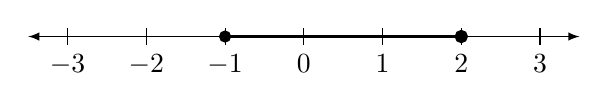
\begin{tikzpicture}
                \draw[very thick] (-1,0) -- (2,0);
                \path [draw=black, fill=black] (-1,0) circle (2pt);
                \path [draw=black, fill=black, thick] (2,0.0) circle (2pt);
                \draw[latex-latex] (-3.5,0) -- (3.5,0) ;
                \foreach \x in  {-3,-2,-1,0,1,2,3}
                \draw[shift={(\x,0)},color=black] (0pt,3pt) -- (0pt,-3pt);
                \foreach \x in {-3,-2,-1,0,1,2,3}
                \draw[shift={(\x,0)},color=black] (0pt,0pt) -- (0pt,-3pt) node[below] 
                {$\x$};
            \end{tikzpicture}
    \end{center}
    \item An open interval does not contain the endpoints. It is represented by $(a,b)$ or $a<x<b$. Similarly, this can be represented on a number line:
    \begin{center}
        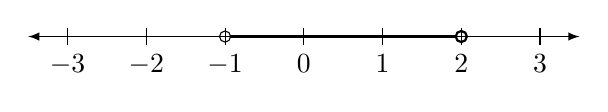
\begin{tikzpicture}
            \draw[very thick] (-1,0) -- (2,0);
            \path [draw=black, fill=white] (-1,0) circle (2pt);
            \path [draw=black, fill=white, thick] (2,0.0) circle (2pt);
            \draw[latex-latex] (-3.5,0) -- (3.5,0) ;
            \foreach \x in  {-3,-2,-1,0,1,2,3}
            \draw[shift={(\x,0)},color=black] (0pt,3pt) -- (0pt,-3pt);
            \foreach \x in {-3,-2,-1,0,1,2,3}
            \draw[shift={(\x,0)},color=black] (0pt,0pt) -- (0pt,-3pt) node[below] 
            {$\x$};
        \end{tikzpicture}
    \end{center}
    \item A half-closed or half-open interval is when only one of the ends are closed, and is denoted by $[a,b)$ or $(a,b]$.
    \item If an interval goes to infinity, such as $(-\infty,b]$ which is equivalent to $x\le b$. Note that this does not imply infinity is a number (or else the interval could be closed), but instead we can define an expression where infinity is embedded into such that it is rigorously logical.
    \begin{center}
        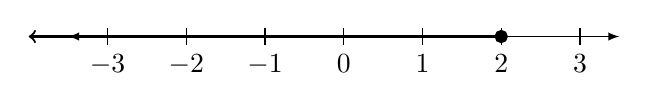
\begin{tikzpicture}
            \draw[<-,thick] (-4,0) -- (2,0);
            % \path [draw=black, fill=white] (-1,0) circle (2pt);
            \path [draw=black, fill=black, thick] (2,0.0) circle (2pt);
            \draw[latex-latex] (-3.5,0) -- (3.5,0) ;
            \foreach \x in  {-3,-2,-1,0,1,2,3}
            \draw[shift={(\x,0)},color=black] (0pt,3pt) -- (0pt,-3pt);
            \foreach \x in {-3,-2,-1,0,1,2,3}
            \draw[shift={(\x,0)},color=black] (0pt,0pt) -- (0pt,-3pt) node[below] 
            {$\x$};
        \end{tikzpicture}
    \end{center}
    \item There are two sets of numbers involved in \textbf{functions}: an x-set and a y-set.
    \begin{definition}
        A function is any \textbf{rule} that assigns each x-number to \emph{one} y-number.
    \end{definition}
    Note that any prescription for the function is acceptable. For example, a table is an example of a function. Neither the x's or y's have to include numbers. There can be holes!
    \item For each x, only a single value of y can be assigned, i.e. double functions are not allowed.\footnote{This is only from how we are defining functions. Other definitions may allow double valued functions.}
    \item Usually we specify functions using an algebraic equation. If for some set of $x$'s, the equation gives a real number $y$, then it is \textit{assumed} that this \textit{specifies} the set of x's for this function. For example:
    \begin{equation}
        f(x)=\begin{cases}
            \frac{10x+5x^2}{x}=10+5x\, & x\neq 0\\ 
            \text{DNE}\, & x = 0
        \end{cases}
        \label{eq:}
    \end{equation}
    This is a perfectly good function since it assigns each number in the $x$-set for this function to some $y$-value.
    \item The \textbf{domain of a function} is the set of x-values and the \textbf{range of a function} as the set of y-values. Here, $x$ is the independent variable and $y$ is the dependent variable.
    
    Note that this doesn't work the other way around, since each $x$ can be used to specify one $y$ but each $y$ can have several corresponding $x$ values! There is some asymmetry involved.
    \item We want to define trigonometric functions purely algebraically, but for now we have to do it geometrically.
    \begin{center}
        \begin{tikzpicture}
            \draw [<->] (-3,0) -- (3,0) node [at end, right] {$x$};
            \draw [<->] (0,-3) -- (0,3) node [at end, left] {$y$};
            \draw[] (0,0) circle (2);

            \draw[thick] (0,0) node[above right,yshift=-0.08cm] {$x$} -- (1,0) node[midway, below] {$\cos x$};
            \draw[thick] (1,0) -- (1,1.732) node[midway, right] {$\sin x$};
            \draw[dotted] (0,0) -- (1,1.732);
        \end{tikzpicture}
    \end{center}
    where the angle is in radians. Radians are picked as the unit such that the arc (curved part subtended by angle of $\theta$) is given by
    \begin{equation}
        s = Rx
        \label{eq:}
    \end{equation}
    where $R$ is the radius of the circle.
    \item Not all algebraic expressions are functions. Suppose we have an ellipse:
    \begin{equation}
        \frac{x^2}{a^2}+\frac{y^2}{b}=1
        \label{eq:}
    \end{equation}
    and solving for $y$ gives:
    \begin{equation}
        y = \pm b\left(1-\frac{x^2}{a^2}\right)^{1/2}
        \label{eq:}
    \end{equation}
    Since we can't have double valued functions, we can instead break this up into \emph{two separate functions}
    \item Composite functions can be written in the form of $f(g(x))$.
    \begin{example}
        Let $f(x)=x^2+2$ and $g(x)=\sin x$. Then:
        \begin{align}
            f(g(x))&=\sin^2(x)+2 \\
            g(f(x))&=\sin(x^2+2)
        \end{align}
        must be true.
    \end{example}
    \item We also need a rigorous way to define \textbf{increasing} and \textbf{decreasing functions}.
    \begin{definition}
        $f(x)$ is increasing on an interval $I$ if $f(x_1)<f(x_2)$ for all $x_1<x_2$ in $I$.\footnote{The motivation behind this definition is to forego the ambiguity when we try to say something like ``As $x$ gets bigger, $y$ gets bigger.'' However a function is a definite relationship between pairs of numbers, none of the values are actually changing! }
    \end{definition}
    Similarly, we can define a decreasing function to be the converse, where $f(x_1)>f(x_2)$ for all $x_1<x_2$ in $I$.\footnote{Note that we can't define an increasing or decreasing function based on its derivative since $y=x^3$ is increasing but it has a derivative of zero at $x=0$.}
    \begin{example}
        Prove that $f(x)=x^2+3$ is increasing for $x>0$.
        \vspace{2mm}

        Consider any two numbers $x_1, x_2$ such that \begin{equation}
            0<x_1<x_2.
            \label{eq:}
        \end{equation}
        Multiplying by $x_1$, we get:
        \begin{equation}
            0<x_1^2<\boxed{x_1x_2}.
            \label{eq:}
        \end{equation}
        We can also multiply by $x_2$, we get:
        \begin{equation}
            0<\boxed{x_1x_2}<x_2^2
            \label{eq:}
        \end{equation}
        Comparing these two inequalities by comparing the boxed compressions, we show that:
        \begin{align}
            x_1^2<x_2^2 \\ 
            x_1^2+3<x_2+3 \\ 
            f(x_1) < f(x_2)
            \label{eq:}
        \end{align}
        Therefore, $f(x)$ is increasing on the interval $x>0$.
    \end{example}
    \begin{example}\label{example:x^2+3 decreasing}
        Prove that $f(x)=x^2+3$ is decreasing for $x<0$.
        \vspace{2mm}

        Consider any two numbers $x_1, x_2$ such that \begin{equation}
            x_1<x_2<0.
        \end{equation}
        Multiplying by $x_1$, we get:
        \begin{equation}
            x_1^2>\boxed{x_1x_2}>0
            \label{eq:}
        \end{equation}
        since we are multiplying by a negative number. We can also multiply by $x_2$ (which is also negative) to get:
        \begin{equation}
            \boxed{x_1x_2}>x_2^2>0
            \label{eq:}
        \end{equation}
        Comparing these two inequalities by comparing the boxed expressions, we show that:
        \begin{align}
            x_1^2>x_2^2 \\ 
            x_1^2+3>x_2+3 \\ 
            f(x_1) > f(x_2)
            \label{eq:}
        \end{align}
        Therefore, $f(x)$ is decreasing on the interval $x<0$.
    \end{example}
    \item We can also define odd and even functions:
    \begin{definition}
        A function $f(x)$ is even if $f(-x)=f(x)$ for all $x$ in the domain of $f(x)$. Similarly, $f(x)$ is odd if $f(-x)=-f(x)$ for all $x$ in the domain of $f(x)$.
    \end{definition}
    \item For arithmetic equalities and inequalities, we are given \textit{arithmetic statements}:
    \begin{itemize}
        \item Equality (e.g. $1+2=6-3$)
        \item Inequality (e.g. $3<5$)
    \end{itemize}
    \begin{theorem}
        You can add, subtract, multiply, or divide both sides by the same factor (positive or negative) and get another true statement.
        \vspace{2mm}

        However, for \emph{inequalities} with a \emph{negative factor} and for \emph{multiplication and division} only, one has to \textit{reverse the sign} of the inequality.\footnote{To convince yourself why this is true, suppose we start with $3<5$ and multiply both sides by $-7$. Is it true that $-21<-35$?}
    \end{theorem}
\end{itemize}